\documentclass[aspectratio=169,11pt]{beamer}

% ── Theme & Colors ──
\usetheme{Madrid}
\usecolortheme{seahorse}
\setbeamertemplate{navigation symbols}{}
\setbeamertemplate{footline}[frame number]
\setbeamerfont{footnote}{size=\tiny}

% ── Packages ──
\usepackage{amsmath,amssymb,amsthm}
\usepackage{mathtools}
\usepackage{booktabs}
\usepackage{tikz}
\usetikzlibrary{arrows.meta,positioning,shapes,calc,fit,backgrounds,decorations.pathreplacing}
\usepackage{xcolor}
\usepackage{pgfplots}
\pgfplotsset{compat=1.17}
\usepackage{hyperref}
\usepackage{appendixnumberbeamer}

% ── Custom Colors ──
\definecolor{dsiorange}{RGB}{255,127,14}
\definecolor{genreblue}{RGB}{31,119,180}
\definecolor{sealgreen}{RGB}{44,160,44}
\definecolor{ncipurple}{RGB}{148,103,189}
\definecolor{lightgray}{RGB}{240,240,240}
\definecolor{darktext}{RGB}{50,50,50}
\definecolor{hybridred}{RGB}{214,39,40}

% ── Macros ──
\newcommand{\vq}{\mathbf{q}}
\newcommand{\vd}{\mathbf{d}}
\newcommand{\vc}{\mathbf{c}}
\newcommand{\R}{\mathbb{R}}
\DeclareMathOperator*{\argmax}{arg\,max}
\DeclareMathOperator*{\argmin}{arg\,min}
\newcommand{\score}{\text{score}}

% ── Notes ──
% For presentation: hide notes in the PDF
\setbeameroption{hide notes}
% To see notes on your screen while presenting, uncomment the line below
% and use pdfpc: pdfpc lecture2_generative_retrieval.pdf
%\setbeameroption{show notes on second screen=right}

% ── Title ──
\title[Generative Retrieval]{Generative Retrieval:\\From Memorization to Generation}
\subtitle{DSI, GENRE, SEAL, and Beyond}
\author{Information Retrieval -- Graduate Seminar}
\date{}

\begin{document}

% ═══════════════════════════════════════════════
% TITLE
% ═══════════════════════════════════════════════
\begin{frame}
\titlepage
\end{frame}

\note{Welcome to the lecture on Generative Retrieval. This is a fundamentally different paradigm from dense retrieval: instead of encoding documents into vectors and searching an index, we train a seq2seq model that directly \emph{generates} document identifiers given a query. We'll cover the key methods (DSI, GENRE, SEAL, NCI), the crucial question of document ID design, theoretical capacity limits, and open challenges.}

% ═══════════════════════════════════════════════
% OUTLINE
% ═══════════════════════════════════════════════
\begin{frame}{Outline}
\tableofcontents
\end{frame}

% ═══════════════════════════════════════════════
\section{Motivation \& Paradigm Shift}
% ═══════════════════════════════════════════════

\begin{frame}[fragile]{The Retrieval Paradigm Landscape}
\begin{center}
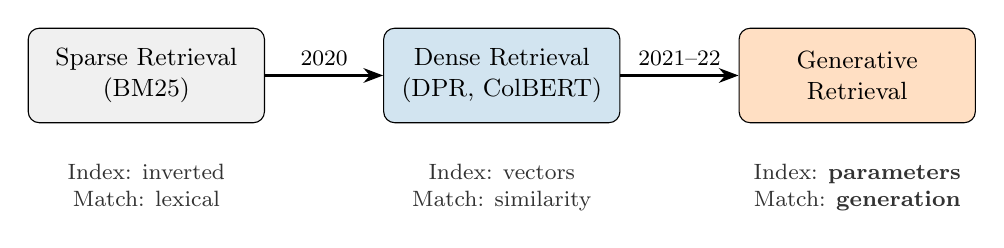
\begin{tikzpicture}[
    box/.style={draw, rounded corners, fill=#1, minimum height=1.2cm, minimum width=3cm, align=center, font=\small},
    arr/.style={-{Stealth[length=2.5mm]}, thick}
]
\node[box=lightgray] (sparse) {Sparse Retrieval\\(BM25)};
\node[box=genreblue!20, right=1.5cm of sparse] (dense) {Dense Retrieval\\(DPR, ColBERT)};
\node[box=dsiorange!25, right=1.5cm of dense] (gen) {Generative\\Retrieval};

\draw[arr] (sparse) -- (dense) node[midway, above, font=\footnotesize] {2020};
\draw[arr] (dense) -- (gen) node[midway, above, font=\footnotesize] {2021--22};

\node[below=0.4cm of sparse, font=\footnotesize, text=darktext, align=center] {Index: inverted\\Match: lexical};
\node[below=0.4cm of dense, font=\footnotesize, text=darktext, align=center] {Index: vectors\\Match: similarity};
\node[below=0.4cm of gen, font=\footnotesize, text=darktext, align=center] {Index: \textbf{parameters}\\Match: \textbf{generation}};
\end{tikzpicture}
\end{center}

\vspace{0.4cm}
\textbf{Key shift}: The entire corpus is encoded into the model's \emph{parameters}. Retrieval becomes \emph{generation}: given a query, generate the identifier of the relevant document.
\end{frame}

\note{This slide frames the paradigm evolution. Sparse retrieval uses inverted indices; dense retrieval uses vector indices. Generative retrieval takes the radical step of encoding the entire corpus into model parameters. Retrieval is then text generation: the model autoregressively produces a document identifier. No external index needed.}

\begin{frame}{Why Generative Retrieval?}
\begin{enumerate}
    \item \textbf{End-to-end differentiable}: Single model replaces separate indexing + retrieval stages.
    \item \textbf{No negative sampling}: Standard seq2seq cross-entropy --- no need to carefully construct negatives.
    \item \textbf{Implicit cross-encoding}: Decoder attends to both query representation and partial docid, enabling richer interaction than bi-encoders.
    \item \textbf{Parametric memory}: Document knowledge stored in weights, not external storage.
\end{enumerate}

\vspace{0.4cm}
\textbf{Central question}: Can a neural network \emph{memorize} an entire corpus well enough to retrieve from it?
\end{frame}

\note{Generative retrieval is appealing because it's a unified end-to-end system. No separate indexing pipeline, no ANN index to maintain, no negative sampling. The model directly learns query-to-document mappings. But this raises a fundamental question about the capacity of neural networks to serve as databases.}

\begin{frame}{Problem Formulation}
\textbf{Two-phase framework}:

\vspace{0.3cm}
\textbf{Phase 1 --- Indexing} (training): Teach the model to memorize documents.
\[
\text{Given } (d_i, c_i) \;\;\text{pairs, learn}\;\; f_\theta : d_i \mapsto c_i
\]
where $d_i$ is document text and $c_i$ is its identifier (docid).

\vspace{0.3cm}
\textbf{Phase 2 --- Retrieval} (inference): Given query $q$, generate the docid.
\[
\hat{c} = \argmax_{c} \; P_\theta(c \mid q) = \argmax_{c} \prod_{t=1}^{|c|} P_\theta(c_t \mid c_{<t}, q)
\]

\vspace{0.3cm}
\textbf{Training data}: $\{(q_i, c_i)\}$ --- query--docid pairs from relevance judgments.
\end{frame}

\note{Formally, generative retrieval has two phases. In indexing, the model learns to map document text to document identifiers. In retrieval, it maps queries to identifiers. The retrieval is autoregressive: the model generates the docid one token at a time, conditioning on the query and previously generated tokens.}

% ═══════════════════════════════════════════════
\section{Foundational Methods}
% ═══════════════════════════════════════════════

\subsection{GENRE: Autoregressive Entity Retrieval}

\begin{frame}[fragile]{GENRE [De Cao et al., ICLR 2021]}
\textbf{First} autoregressive approach to entity retrieval.

\vspace{0.3cm}
\begin{center}
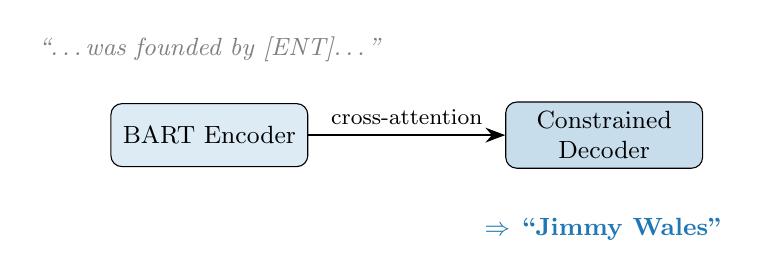
\begin{tikzpicture}[
    box/.style={draw, rounded corners, fill=#1, minimum height=0.8cm, minimum width=2.5cm, align=center, font=\small},
    arr/.style={-{Stealth[length=2.5mm]}, thick}
]
\node[box=genreblue!15] (enc) {BART Encoder};
\node[box=genreblue!25, right=2.5cm of enc] (dec) {Constrained\\Decoder};
\node[above=0.4cm of enc, font=\small\itshape, text=gray] {``\ldots was founded by [ENT]\ldots''};
\node[below=0.5cm of dec, font=\small\bfseries, text=genreblue] {$\Rightarrow$ ``Jimmy Wales''};

\draw[arr] (enc) -- (dec) node[midway, above, font=\footnotesize] {cross-attention};
\end{tikzpicture}
\end{center}

\vspace{0.3cm}
\textbf{Key innovations}:
\begin{itemize}
    \item Entity \emph{names} serve as identifiers (natural language, not integers).
    \item \textbf{Constrained beam search}: At each step, only tokens that extend a valid entity name are allowed.
    \item Fine-tuned BART (denoising seq2seq pre-training).
\end{itemize}
\end{frame}

\note{GENRE was the pioneering work. It showed that you can generate entity names autoregressively from context. The key trick is constrained beam search: the decoder is only allowed to produce token sequences that correspond to valid entity names in a predefined vocabulary. This eliminates hallucinated entities. GENRE achieved SOTA on 20+ entity linking and disambiguation datasets.}

\begin{frame}[fragile]{GENRE: Constrained Beam Search}
\begin{center}
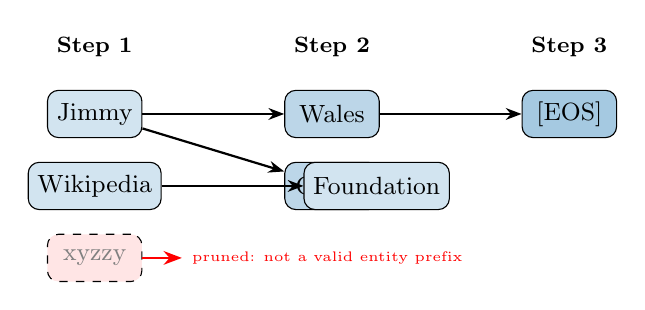
\begin{tikzpicture}[
    node distance=0.8cm and 1.5cm,
    tok/.style={draw, rounded corners, fill=#1, minimum width=1.2cm, minimum height=0.6cm, font=\small},
    pruned/.style={draw, rounded corners, fill=red!10, minimum width=1.2cm, minimum height=0.6cm, font=\small, dashed, text=gray},
    arr/.style={-{Stealth[length=2mm]}, thick}
]
% Step 1
\node[tok=genreblue!20] (j) {Jimmy};
\node[tok=genreblue!20, below=0.3cm of j] (w) {Wikipedia};
\node[pruned, below=0.3cm of w] (x) {xyzzy};

% Step 2
\node[tok=genreblue!30, right=1.8cm of j] (jw) {Wales};
\node[tok=genreblue!30, below=0.3cm of jw] (jc) {Carter};
\node[tok=genreblue!20, right=1.8cm of w] (wf) {Foundation};

% Step 3
\node[tok=genreblue!40, right=1.8cm of jw] (jwe) {[EOS]};

\draw[arr] (j) -- (jw);
\draw[arr] (j) -- (jc);
\draw[arr] (w) -- (wf);
\draw[arr] (jw) -- (jwe);

% Labels
\node[above=0.3cm of j, font=\footnotesize\bfseries] {Step 1};
\node[above=0.3cm of jw, font=\footnotesize\bfseries] {Step 2};
\node[above=0.3cm of jwe, font=\footnotesize\bfseries] {Step 3};

% Pruning annotation
\draw[thick, red, -{Stealth}] (x.east) -- ++(0.5,0) node[right, font=\tiny, text=red] {pruned: not a valid entity prefix};
\end{tikzpicture}
\end{center}

\vspace{0.3cm}
At each decoding step, maintain a \textbf{trie} of valid entity names. Only tokens that extend a valid prefix are kept in the beam.

\vspace{0.2cm}
\textbf{Result}: Exact softmax over entity vocabulary --- no negative sampling needed.
\end{frame}

\note{The constrained beam search works by maintaining a trie of all valid entity names. At each step, the decoder proposes tokens, but only those extending a valid prefix in the trie survive. Invalid continuations are pruned. This means the model's output is always a valid entity, and the loss is an exact cross-entropy over the valid set---no sampling approximation needed.}

\subsection{DSI: Differentiable Search Index}

\begin{frame}[fragile]{DSI: Core Idea [Tay et al., NeurIPS 2022]}
\textbf{Vision}: Encode the entire corpus into a Transformer's parameters.

\vspace{0.4cm}
\begin{center}
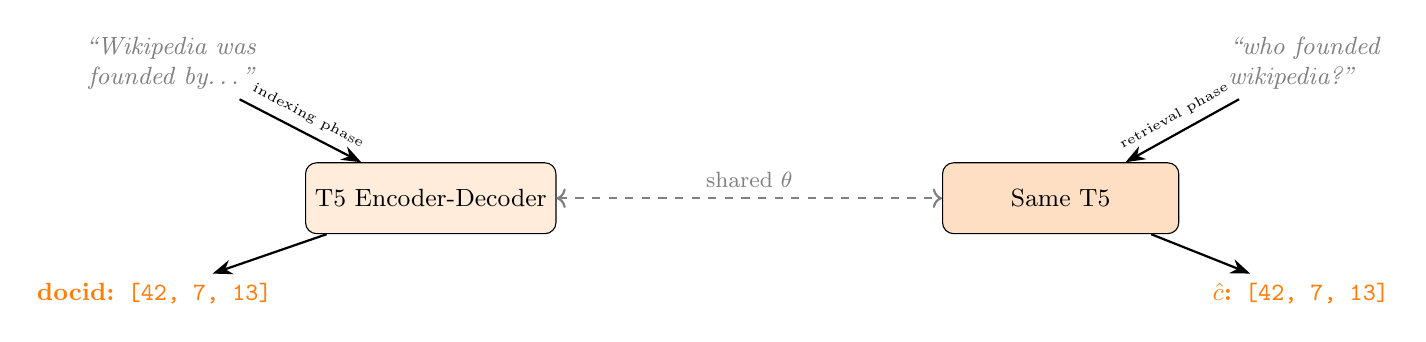
\begin{tikzpicture}[
    box/.style={draw, rounded corners, fill=#1, minimum height=0.9cm, minimum width=3cm, align=center, font=\small},
    arr/.style={-{Stealth[length=2.5mm]}, thick}
]
% Indexing
\node[box=dsiorange!15] (idx) at (0,0) {T5 Encoder-Decoder};
\node[above left=0.8cm and 0.5cm of idx, font=\small\itshape, text=gray, align=right] (doc) {``Wikipedia was\\founded by\ldots''};
\node[below left=0.5cm and 0.3cm of idx, font=\small\bfseries, text=dsiorange] (cid) {docid: \texttt{[42, 7, 13]}};

\draw[arr] (doc) -- (idx) node[midway, above, font=\tiny, sloped] {indexing phase};
\draw[arr] (idx) -- (cid);

% Retrieval
\node[box=dsiorange!25] (ret) at (8,0) {Same T5};
\node[above right=0.8cm and 0.5cm of ret, font=\small\itshape, text=gray, align=left] (query) {``who founded\\wikipedia?''};
\node[below right=0.5cm and 0.3cm of ret, font=\small\bfseries, text=dsiorange] (rid) {$\hat{c}$: \texttt{[42, 7, 13]}};

\draw[arr] (query) -- (ret) node[midway, above, font=\tiny, sloped] {retrieval phase};
\draw[arr] (ret) -- (rid);

\draw[thick, dashed, gray, <->] (idx) -- (ret) node[midway, above, font=\footnotesize] {shared $\theta$};
\end{tikzpicture}
\end{center}

\vspace{0.3cm}
\textbf{Two tasks, one model}:
\begin{enumerate}
    \item \textbf{Indexing}: $P_\theta(\text{docid} \mid \text{document})$ --- memorize the corpus.
    \item \textbf{Retrieval}: $P_\theta(\text{docid} \mid \text{query})$ --- retrieve given a query.
\end{enumerate}
\end{frame}

\note{DSI's vision is radical: a single T5 model serves as both the index and the retriever. During indexing, the model learns to map document text to document identifiers. During retrieval, it maps queries to identifiers. Both are seq2seq tasks sharing the same parameters. The corpus is literally encoded in the model's weights.}

\begin{frame}{DSI: Document ID Design Space}
\textbf{The central design question}: How to assign identifiers to documents?

\vspace{0.4cm}
\begin{center}
\begin{tabular}{lp{5cm}c}
\toprule
\textbf{Strategy} & \textbf{Description} & \textbf{Example} \\
\midrule
Unstructured (atomic) & One unique token per document & \texttt{[DOC\_42]} \\
\addlinespace
Naively structured & Arbitrary integer sequence & \texttt{[4, 2, 7, 1]} \\
\addlinespace
Semantically structured & Hierarchical clustering path & \texttt{[C3, C7, C2]} \\
\bottomrule
\end{tabular}
\end{center}

\vspace{0.4cm}
\textbf{Surprising finding}: Semantically structured IDs do \emph{not} consistently outperform unstructured ones. The Transformer can learn arbitrary mappings regardless of ID structure.
\end{frame}

\note{DSI explored three document ID strategies. Atomic IDs add one new vocabulary token per document. Naive structured IDs use sequences of existing integers. Semantic structured IDs use hierarchical k-means clustering paths. The surprising result was that atomic IDs often worked as well as semantic ones. This suggests Transformers are powerful enough to learn arbitrary query-to-ID mappings, and the ID structure matters less than one might expect.}

\begin{frame}{DSI: Semantic Document IDs via Hierarchical Clustering}
\begin{center}
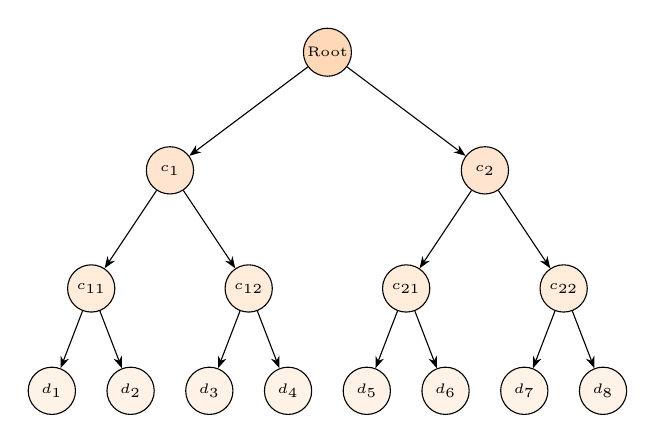
\begin{tikzpicture}[
    level 1/.style={sibling distance=4cm, level distance=1.5cm},
    level 2/.style={sibling distance=2cm, level distance=1.5cm},
    level 3/.style={sibling distance=1cm, level distance=1.3cm},
    every node/.style={draw, circle, minimum size=0.6cm, font=\tiny, inner sep=1pt},
    edge from parent/.style={draw, -{Stealth[length=1.5mm]}},
]
\node[fill=dsiorange!30] {Root}
    child {node[fill=dsiorange!20] {$c_1$}
        child {node[fill=dsiorange!15] {$c_{11}$}
            child {node[fill=dsiorange!10] {$d_1$}}
            child {node[fill=dsiorange!10] {$d_2$}}
        }
        child {node[fill=dsiorange!15] {$c_{12}$}
            child {node[fill=dsiorange!10] {$d_3$}}
            child {node[fill=dsiorange!10] {$d_4$}}
        }
    }
    child {node[fill=dsiorange!20] {$c_2$}
        child {node[fill=dsiorange!15] {$c_{21}$}
            child {node[fill=dsiorange!10] {$d_5$}}
            child {node[fill=dsiorange!10] {$d_6$}}
        }
        child {node[fill=dsiorange!15] {$c_{22}$}
            child {node[fill=dsiorange!10] {$d_7$}}
            child {node[fill=dsiorange!10] {$d_8$}}
        }
    };
\end{tikzpicture}
\end{center}

\vspace{0.2cm}
\textbf{Construction}:
\begin{enumerate}
    \item Embed all documents with pre-trained encoder (e.g., BERT).
    \item Recursive $k$-means clustering on embeddings.
    \item Each document's ID = path from root: e.g., $d_3 \to [c_1, c_{12}, 1]$.
\end{enumerate}

\textbf{Intuition}: Semantically similar documents share ID prefixes $\Rightarrow$ the decoder can progressively narrow its search.
\end{frame}

\note{Semantic IDs are built by hierarchically clustering document embeddings. Documents in the same cluster share a prefix. The idea is that the decoder first generates the coarse cluster, then refines. However, experiments showed this hierarchy doesn't always help: the Transformer can learn arbitrary structures. Still, semantic IDs are a widely studied design choice.}

\begin{frame}{DSI: Training Objective}
\textbf{Multi-task training}: Jointly learn indexing and retrieval.

\vspace{0.3cm}
\begin{block}{Indexing Loss (Memorization)}
\vspace{-0.3cm}
\[
\mathcal{L}_{\text{index}} = -\sum_{(d_i, c_i)} \sum_{t=1}^{|c_i|} \log P_\theta\bigl(c_{i,t} \mid c_{i,<t},\, d_i\bigr)
\]
\end{block}

\begin{block}{Retrieval Loss}
\vspace{-0.3cm}
\[
\mathcal{L}_{\text{retrieve}} = -\sum_{(q_i, c_i)} \sum_{t=1}^{|c_i|} \log P_\theta\bigl(c_{i,t} \mid c_{i,<t},\, q_i\bigr)
\]
\end{block}

\[
\mathcal{L}_{\text{DSI}} = \mathcal{L}_{\text{index}} + \lambda \cdot \mathcal{L}_{\text{retrieve}}
\]

\textbf{Note}: Both are standard cross-entropy losses --- no negative sampling required.
\end{frame}

\note{DSI trains with two losses. The indexing loss teaches the model to map documents to their IDs (memorization). The retrieval loss teaches it to map queries to IDs (generalization). Both are standard cross-entropy. A key advantage over dense retrieval: no negative sampling needed. The softmax over the vocabulary serves as an implicit normalization.}

\subsection{SEAL: N-gram Identifiers}

\begin{frame}{SEAL: Substrings as Document Identifiers [Bevilacqua et al., NeurIPS 2022]}
\textbf{Key insight}: Use \emph{all} n-grams from a document as potential identifiers.

\vspace{0.3cm}
\begin{center}
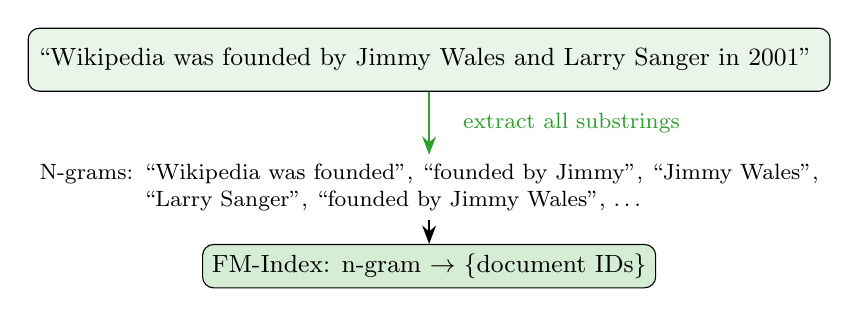
\begin{tikzpicture}[font=\small]
\node[draw, rounded corners, fill=sealgreen!10, minimum width=10cm, minimum height=0.8cm, align=center] (doc) {
    ``Wikipedia was founded by Jimmy Wales and Larry Sanger in 2001''
};

\node[below=0.8cm of doc, font=\footnotesize, align=left] (ngrams) {
    N-grams: ``Wikipedia was founded'', ``founded by Jimmy'', ``Jimmy Wales'', \\
    \phantom{N-grams: }``Larry Sanger'', ``founded by Jimmy Wales'', \ldots
};

\draw[-{Stealth}, thick, sealgreen] (doc) -- (ngrams) node[midway, right, xshift=0.3cm, font=\footnotesize] {extract all substrings};

\node[below=0.3cm of ngrams, draw, rounded corners, fill=sealgreen!20, font=\small] (fm) {FM-Index: n-gram $\to$ \{document IDs\}};
\draw[-{Stealth}, thick] (ngrams) -- (fm);
\end{tikzpicture}
\end{center}

\vspace{0.2cm}
\textbf{Advantage}: Identifiers are \emph{natural language substrings} $\Rightarrow$ leverage pre-trained LM knowledge. No need to engineer an ID space.
\end{frame}

\note{SEAL takes a radically different approach to document IDs. Instead of assigning artificial identifiers, it uses all n-grams from the document as valid IDs. So ``Jimmy Wales and Larry Sanger'' is a valid identifier for the Wikipedia article. This leverages the language model's pre-trained knowledge of natural language substrings. The FM-Index efficiently maps any substring to its containing documents.}

\begin{frame}{SEAL: FM-Index \& Constrained Decoding}
\textbf{FM-Index}: Compressed full-text substring index based on Burrows-Wheeler Transform.
\begin{itemize}
    \item Space: $\sim$7$\times$ smaller than DPR embedding index.
    \item Lookup: Given partial n-gram, returns valid continuations.
\end{itemize}

\vspace{0.3cm}
\textbf{Decoding process}:
\begin{enumerate}
    \item Generate n-gram tokens autoregressively (BART decoder).
    \item At each step, FM-Index constrains valid next tokens.
    \item Multiple n-grams per query $\Rightarrow$ aggregate scores across n-grams.
\end{enumerate}

\vspace{0.3cm}
\textbf{Scoring}:
\[
\score(q, d) = \sum_{g \in \text{generated n-grams}} P_\theta(g \mid q) \cdot \mathbf{1}[g \in d]
\]

Aggregate generation probability of n-grams that appear in document $d$.
\end{frame}

\note{The FM-Index is the critical data structure. Based on the Burrows-Wheeler Transform, it compresses all substrings into a space-efficient index. During decoding, it tells the model which tokens are valid continuations of the current n-gram prefix. This ensures every generated n-gram actually appears in the corpus. Multiple n-grams are generated per query, and their probabilities are aggregated to score documents.}

\subsection{NCI: Neural Corpus Indexer}

\begin{frame}{NCI: Key Contributions [Wang et al., NeurIPS 2022]}
\begin{enumerate}
    \item \textbf{Prefix-Aware Weight-Adaptive Decoder}:
    \begin{itemize}
        \item Standard decoder treats each token independently.
        \item NCI dynamically adjusts decoder weights based on the generated prefix.
        \item If prefix $= [c_1, c_2]$, the decoder is ``aware'' it's generating at level 3 of the hierarchy.
    \end{itemize}

    \vspace{0.3cm}
    \item \textbf{Query Generation for Data Augmentation}:
    \begin{itemize}
        \item Use DocT5Query to generate synthetic queries per document.
        \item Creates $K$ pseudo query--docid pairs per document.
        \item Critical for scaling to large corpora where labeled queries are sparse.
    \end{itemize}

    \vspace{0.3cm}
    \item \textbf{Consistency Regularization}:
    \[
    \mathcal{L}_{\text{consist}} = \text{KL}\bigl(P_\theta(c \mid q_1) \;\|\; P_\theta(c \mid q_2)\bigr)
    \]
    where $q_1, q_2$ are different queries for the same document.
\end{enumerate}
\end{frame}

\note{NCI improves on DSI in three ways. First, the prefix-aware decoder adapts its weights depending on what it has already generated, which is crucial for hierarchical IDs. Second, it uses DocT5Query to generate synthetic queries, massively expanding the training data. Third, consistency regularization ensures the model produces the same docid for semantically similar queries, reducing noise from the synthetic data.}

\begin{frame}{NCI: Results}
\begin{center}
\begin{tabular}{lcc}
\toprule
\textbf{Method} & \textbf{NQ320K R@1} & \textbf{NQ320K R@10} \\
\midrule
BM25 & 12.4 & 38.3 \\
DPR & 30.1 & 63.1 \\
DSI (T5-base) & 27.4 & 56.6 \\
\textbf{NCI} & \textbf{51.5} & \textbf{77.9} \\
\bottomrule
\end{tabular}
\end{center}

\vspace{0.4cm}
\textbf{+21.4\% R@1 over best baseline.}

\vspace{0.3cm}
The gains come primarily from:
\begin{itemize}
    \item Query augmentation ($\sim$60\% of the gain)
    \item Prefix-aware decoder ($\sim$25\%)
    \item Consistency regularization ($\sim$15\%)
\end{itemize}
\end{frame}

\note{NCI delivers dramatic improvements. On NQ320K, it nearly doubles DPR's Recall@1. The ablation shows that query augmentation is the single biggest contributor. This makes sense: generative retrieval requires the model to memorize query-to-docid mappings, and more diverse queries during training lead to better generalization.}

% ═══════════════════════════════════════════════
\section{The Document ID Design Space}
% ═══════════════════════════════════════════════

\begin{frame}[fragile]{Document ID Design: Three Dimensions}
\begin{center}
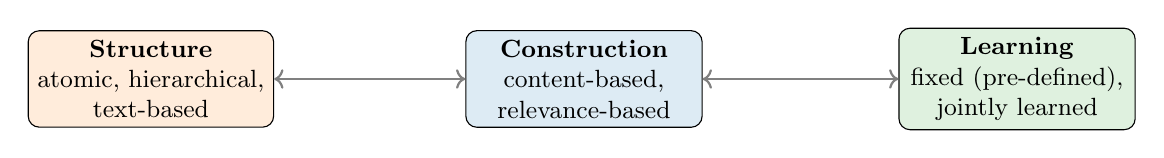
\begin{tikzpicture}[
    dim/.style={draw, rounded corners, fill=#1, minimum width=3cm, minimum height=1cm, align=center, font=\small},
]
\node[dim=dsiorange!15] (struct) at (0,0) {\textbf{Structure}\\atomic, hierarchical,\\text-based};
\node[dim=genreblue!15] (construct) at (5.5,0) {\textbf{Construction}\\content-based,\\relevance-based};
\node[dim=sealgreen!15] (learn) at (11,0) {\textbf{Learning}\\fixed (pre-defined),\\jointly learned};

\draw[thick, <->, gray] (struct) -- (construct);
\draw[thick, <->, gray] (construct) -- (learn);
\end{tikzpicture}
\end{center}

\vspace{0.5cm}
\begin{center}
\begin{tabular}{llll}
\toprule
\textbf{Method} & \textbf{Structure} & \textbf{Construction} & \textbf{Example ID} \\
\midrule
DSI (atomic) & Unstructured & Arbitrary & \texttt{[DOC\_42]} \\
DSI (semantic) & Hierarchical & Content (k-means) & \texttt{[3, 7, 2]} \\
GENRE & Text-based & Entity names & ``Jimmy Wales'' \\
SEAL & Text-based & Content (n-grams) & ``founded Wikipedia'' \\
NCI & Hierarchical & Content (clustering) & \texttt{[C5, C12, D3]} \\
\bottomrule
\end{tabular}
\end{center}
\end{frame}

\note{Document ID design has three dimensions: structure (what shape the ID takes), construction (how it's built), and learning (whether it's fixed or learned jointly). Each major method makes different choices. GENRE and SEAL use natural language text, which leverages pre-trained knowledge. DSI and NCI use numeric/hierarchical IDs. The choice profoundly affects both training dynamics and retrieval quality.}

\begin{frame}{Text-Based vs.\ Numeric IDs: A Comparison}
\begin{columns}[T]
\column{0.48\textwidth}
\textbf{Text-Based IDs} (GENRE, SEAL)

\vspace{0.2cm}
\textcolor{sealgreen}{\bfseries Advantages:}
\begin{itemize}
    \item Leverage pre-trained LM knowledge
    \item Semantically meaningful
    \item Better zero-shot generalization
    \item No ID assignment preprocessing
\end{itemize}

\vspace{0.2cm}
\textcolor{hybridred}{\bfseries Disadvantages:}
\begin{itemize}
    \item Larger decoding space
    \item Constrained decoding needed
    \item Multiple IDs per document
\end{itemize}

\column{0.48\textwidth}
\textbf{Numeric/Hierarchical IDs} (DSI, NCI)

\vspace{0.2cm}
\textcolor{sealgreen}{\bfseries Advantages:}
\begin{itemize}
    \item Compact decoding space
    \item One-to-one mapping
    \item Efficient beam search
    \item Hierarchical structure exploitable
\end{itemize}

\vspace{0.2cm}
\textcolor{hybridred}{\bfseries Disadvantages:}
\begin{itemize}
    \item No pre-trained knowledge
    \item Requires clustering pipeline
    \item Arbitrary structure must be learned
\end{itemize}
\end{columns}

\vspace{0.3cm}
\textbf{Recent trend}: Summary-based IDs (keyphrases, abstracts) achieve +15\% recall over cluster IDs.
\end{frame}

\note{There's a real tension in ID design. Text-based IDs benefit from pre-training---the model already knows about ``Jimmy Wales''---but the decoding space is large. Numeric IDs are compact but the model must learn arbitrary mappings from scratch. Recent work on summary-based IDs tries to get the best of both: semantically meaningful but more compact than full n-grams.}

\begin{frame}[fragile]{Document ID Design: Relevance-Based IDs (2024)}
\textbf{New direction}: Construct IDs based on query--document \emph{relevance}, not just content.

\vspace{0.3cm}
\begin{center}
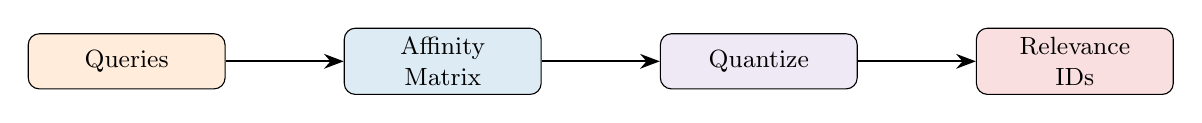
\begin{tikzpicture}[
    box/.style={draw, rounded corners, fill=#1, minimum height=0.7cm, minimum width=2.5cm, align=center, font=\small},
    arr/.style={-{Stealth[length=2.5mm]}, thick}
]
\node[box=dsiorange!15] (q) {Queries};
\node[box=genreblue!15, right=1.5cm of q] (aff) {Affinity\\Matrix};
\node[box=ncipurple!15, right=1.5cm of aff] (quant) {Quantize};
\node[box=hybridred!15, right=1.5cm of quant] (id) {Relevance\\IDs};

\draw[arr] (q) -- (aff);
\draw[arr] (aff) -- (quant);
\draw[arr] (quant) -- (id);
\end{tikzpicture}
\end{center}

\vspace{0.3cm}
\textbf{Idea}: Documents relevant to similar queries should have similar IDs.
\[
\text{ID}(d) = \text{Quantize}\!\left(\sum_{q \in Q_d} \text{relevance}(q, d) \cdot \vq\right)
\]

\vspace{0.2cm}
\textbf{Result}: Better ranking alignment than content-based clustering, because the ID space is optimized for the retrieval task itself.
\end{frame}

\note{Relevance-based IDs are a recent innovation. Instead of clustering documents by content similarity, you cluster by relevance similarity: documents that answer the same kinds of queries get similar IDs. This directly aligns the ID space with the retrieval objective, and experiments show significant improvements over content-based clustering.}

% ═══════════════════════════════════════════════
\section{Recent Advances (2023--2025)}
% ═══════════════════════════════════════════════

\begin{frame}[fragile]{MINDER: Multi-View Identifiers [Li et al., ACL 2023]}
\textbf{Observation}: A single ID type is a bottleneck. Different aspects of a document are best captured by different identifiers.

\vspace{0.4cm}
\begin{center}
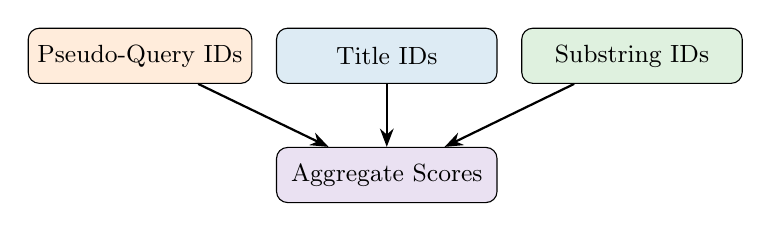
\begin{tikzpicture}[
    box/.style={draw, rounded corners, fill=#1, minimum width=2.8cm, minimum height=0.7cm, align=center, font=\small},
]
\node[box=dsiorange!15] (pq) {Pseudo-Query IDs};
\node[box=genreblue!15, right=0.3cm of pq] (title) {Title IDs};
\node[box=sealgreen!15, right=0.3cm of title] (sub) {Substring IDs};

\node[box=ncipurple!20, below=0.8cm of title] (agg) {Aggregate Scores};

\draw[-{Stealth}, thick] (pq) -- (agg);
\draw[-{Stealth}, thick] (title) -- (agg);
\draw[-{Stealth}, thick] (sub) -- (agg);
\end{tikzpicture}
\end{center}

\vspace{0.3cm}
\textbf{Three views}:
\begin{enumerate}
    \item \textbf{Pseudo-query IDs}: Generated queries (what users might search).
    \item \textbf{Title IDs}: Document titles (concise summaries).
    \item \textbf{Substring IDs}: Key n-grams (fine-grained content).
\end{enumerate}

Multiple views provide redundancy and cross-checking $\Rightarrow$ more robust retrieval.
\end{frame}

\note{MINDER uses three types of identifiers per document simultaneously. The model generates all three types and aggregates their scores. This is analogous to ensemble methods: each view captures different aspects of relevance, and combining them is more robust than any single view.}

\begin{frame}{LTRGR: Learning to Rank in Generative Retrieval [Li et al., AAAI 2023]}
\textbf{Problem}: Standard cross-entropy optimizes \emph{likelihood}, not \emph{ranking quality}.

\vspace{0.3cm}
\begin{center}
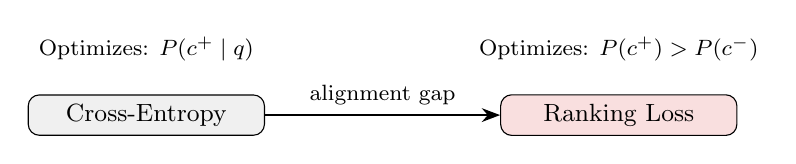
\begin{tikzpicture}[font=\small]
\node[draw, rounded corners, fill=lightgray, minimum width=3cm] (ce) at (0,0) {Cross-Entropy};
\node[draw, rounded corners, fill=hybridred!15, minimum width=3cm] (rank) at (6,0) {Ranking Loss};
\node[above=0.3cm of ce, font=\footnotesize] {Optimizes: $P(c^+ \mid q)$};
\node[above=0.3cm of rank, font=\footnotesize] {Optimizes: $P(c^+) > P(c^-)$};
\draw[thick, -{Stealth}] (ce) -- (rank) node[midway, above, font=\footnotesize] {alignment gap};
\end{tikzpicture}
\end{center}

\vspace{0.3cm}
\textbf{LTRGR adds a pairwise ranking loss}:
\[
\mathcal{L}_{\text{rank}} = -\log \sigma\!\bigl(\log P_\theta(c^+ \mid q) - \log P_\theta(c^- \mid q)\bigr)
\]

\textbf{Combined objective}:
\[
\mathcal{L} = \mathcal{L}_{\text{CE}} + \alpha \cdot \mathcal{L}_{\text{rank}}
\]

\textbf{Result}: Better alignment between generation probability and ranking quality.
\end{frame}

\note{A fundamental issue with generative retrieval is that cross-entropy loss optimizes the probability of generating the correct docid, but doesn't directly optimize ranking. LTRGR adds a pairwise ranking loss that explicitly requires the model to assign higher probability to relevant docids than irrelevant ones. This bridges the gap between generation and ranking objectives.}

\begin{frame}[fragile]{GDR: Generative Dense Retrieval --- Hybrid Approach [2024]}
\textbf{Insight}: Pure memorization has fundamental limits.

\vspace{0.2cm}
\begin{center}
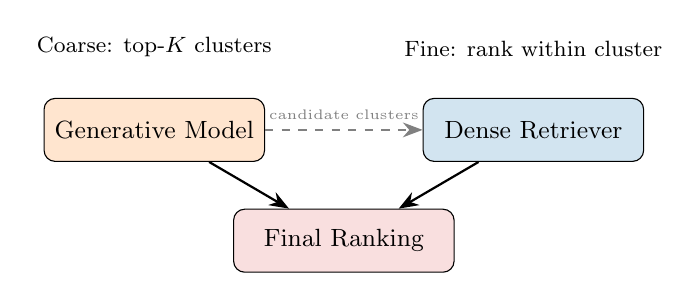
\begin{tikzpicture}[
    box/.style={draw, rounded corners, fill=#1, minimum height=0.8cm, minimum width=2.8cm, align=center, font=\small},
    arr/.style={-{Stealth[length=2.5mm]}, thick}
]
\node[box=dsiorange!20] (gen) {Generative Model};
\node[box=genreblue!20, right=2cm of gen] (dense) {Dense Retriever};
\node[box=hybridred!15, below=1cm of $(gen)!0.5!(dense)$] (final) {Final Ranking};

\node[above=0.4cm of gen, font=\footnotesize] {Coarse: top-$K$ clusters};
\node[above=0.4cm of dense, font=\footnotesize] {Fine: rank within cluster};

\draw[arr] (gen) -- (final);
\draw[arr] (dense) -- (final);
\draw[arr, dashed, gray] (gen) -- (dense) node[midway, above, font=\tiny] {candidate clusters};
\end{tikzpicture}
\end{center}

\vspace{0.3cm}
\textbf{Two-stage pipeline}:
\begin{enumerate}
    \item \textbf{Generative stage}: Model generates top-$K$ cluster IDs (coarse retrieval, using parametric memory).
    \item \textbf{Dense stage}: Standard dense retrieval within selected clusters (fine-grained ranking).
\end{enumerate}

\vspace{0.2cm}
Combines memorization strength (global structure) with embedding strength (local precision).
\end{frame}

\note{GDR recognizes that pure generative retrieval struggles with fine-grained distinctions at large scale. Its solution: use the generative model for coarse-grained cluster selection (where memorization works well), then switch to dense retrieval for precise ranking within clusters (where embeddings excel). This hybrid approach scales much better to large corpora.}

% ═══════════════════════════════════════════════
\section{Theoretical Foundations}
% ═══════════════════════════════════════════════

\begin{frame}{Model Capacity \& Memorization Limits}
\textbf{Fundamental question}: How many documents can a Transformer memorize?

\vspace{0.3cm}
\textbf{Three memorization challenges}:
\begin{enumerate}
    \item \textbf{Poor memory accuracy}: Fine-grained features are poorly memorized as corpus grows.
    \item \textbf{Memory confusion}: Similar documents $\to$ similar representations $\to$ retrieval errors.
    \item \textbf{Update costs}: Adding new documents requires retraining (expensive).
\end{enumerate}

\vspace{0.4cm}
\textbf{Empirical scaling}:
\begin{center}
\begin{tabular}{lcc}
\toprule
\textbf{Corpus Size} & \textbf{Model Size Needed} & \textbf{Approach} \\
\midrule
100K docs & $\sim$100M params & Pure generative \\
1M docs & $\sim$250M params & Generative (with augmentation) \\
10M docs & $\sim$1B params & Hybrid recommended \\
100M+ docs & ??? & Hybrid required \\
\bottomrule
\end{tabular}
\end{center}
\end{frame}

\note{Memorization capacity is the elephant in the room for generative retrieval. Current models work well up to about 1 million documents. Beyond that, memorization quality degrades. At 10 million documents, hybrid approaches become necessary. At web scale (billions), pure generative retrieval is currently infeasible. The scaling isn't linear: you need disproportionately more parameters as the corpus grows.}

\begin{frame}{Memorization vs.\ Generalization}
\textbf{Training dynamics of neural networks} (Arpit et al., 2017):

\vspace{0.3cm}
\begin{center}
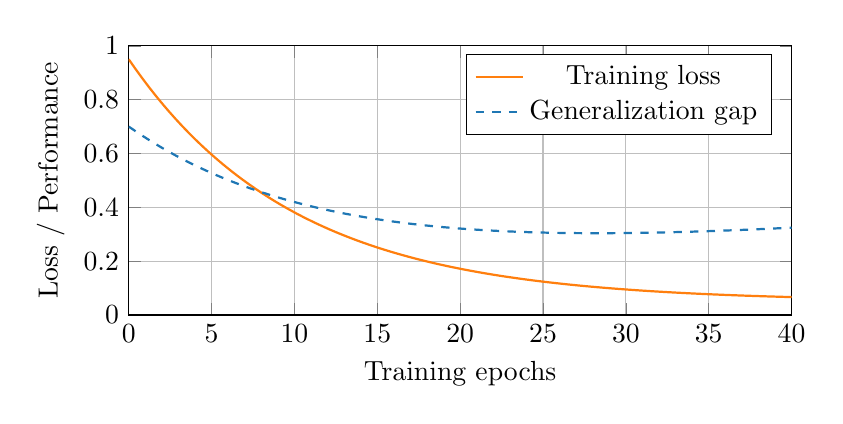
\begin{tikzpicture}
\begin{axis}[
    width=10cm, height=5cm,
    xlabel={Training epochs}, ylabel={Loss / Performance},
    legend pos=north east,
    grid=major,
    xmin=0, xmax=40,
    ymin=0, ymax=1
]
\addplot[dsiorange, thick, domain=0:40, samples=100] {0.9*exp(-0.1*x) + 0.05};
\addlegendentry{Training loss}
\addplot[genreblue, thick, dashed, domain=0:40, samples=100] {0.6*exp(-0.08*x) + 0.1 + 0.005*x};
\addlegendentry{Generalization gap}
\end{axis}
\end{tikzpicture}
\end{center}

\vspace{0.1cm}
\begin{itemize}
    \item \textbf{Phase 1} (early): Model learns generalizable patterns (semantic matching).
    \item \textbf{Phase 2} (late): Model memorizes specific query--docid mappings.
    \item \textbf{Risk}: Over-memorization $\Rightarrow$ poor generalization to unseen queries.
\end{itemize}
\end{frame}

\note{Generative retrieval faces a fundamental tension. Early in training, the model learns general semantic patterns---these generalize well. Later, it memorizes specific query-document associations---these are needed for retrieval but can overfit. The challenge is balancing memorization (needed to store the corpus) with generalization (needed to handle novel queries). Pre-training and query augmentation help maintain this balance.}

\begin{frame}{Retrieval as Generation vs.\ Ranking: A Formal Comparison}
\begin{columns}[T]
\column{0.48\textwidth}
\textbf{Dense Retrieval}:
\[
\mathcal{L}_{\text{dense}} = -\log \frac{e^{\vq^\top \vd^+ / \tau}}{\sum_{j} e^{\vq^\top \vd_j / \tau}}
\]

\begin{itemize}
    \item Locally normalized (over document set)
    \item Requires explicit negatives
    \item External index stores $\{\vd_j\}$
    \item Inference: ANN search
\end{itemize}

\column{0.48\textwidth}
\textbf{Generative Retrieval}:
\[
\mathcal{L}_{\text{gen}} = -\sum_{t} \log P_\theta(c_t \mid c_{<t}, q)
\]

\begin{itemize}
    \item Token-level cross-entropy
    \item No explicit negatives
    \item Parametric memory (weights)
    \item Inference: beam search
\end{itemize}
\end{columns}

\vspace{0.4cm}
\textbf{Theoretical connection}: Under certain decompositions, generative retrieval can be viewed as an implicit bi-encoder where the ``document embedding'' is encoded in the decoder's generation probabilities.
\end{frame}

\note{Let's compare the two paradigms formally. Dense retrieval uses a contrastive loss requiring explicit negatives and an external index. Generative retrieval uses standard cross-entropy with no explicit negatives and parametric storage. Interestingly, recent work has shown that under certain conditions, the two can be connected: generative probabilities implicitly define a similarity function between queries and documents.}

\begin{frame}{Information-Theoretic Perspective on Document IDs}
\textbf{Document IDs as compression codes}:

\vspace{0.3cm}
\begin{itemize}
    \item A docid $c(d)$ is a lossy compression of document $d$.
    \item \textbf{Rate}: $|c(d)|$ --- length of the docid (bits needed).
    \item \textbf{Distortion}: Retrieval error when using $c(d)$ instead of full $d$.
\end{itemize}

\vspace{0.3cm}
\textbf{Rate--Distortion trade-off}:
\[
\min \;\mathbb{E}[\text{retrieval error}] \quad\text{s.t.}\quad \mathbb{E}[|c(d)|] \leq R
\]

\vspace{0.3cm}
\begin{itemize}
    \item \textbf{Short IDs}: Fast decoding, but higher retrieval error (less information).
    \item \textbf{Long IDs}: Lower error, but slower decoding (more beam search steps).
    \item \textbf{Optimal}: Depends on corpus size and model capacity.
\end{itemize}

\vspace{0.2cm}
\textbf{Open question}: Can we derive information-theoretic bounds on optimal docid length?
\end{frame}

\note{From an information-theoretic perspective, a document ID is a lossy code for the document. There's a rate-distortion tradeoff: longer IDs preserve more information but take more decoding steps. Shorter IDs are faster to generate but may lose distinguishing features. This connects to source coding theory, and finding the optimal ID length for a given corpus size is an open theoretical question.}

% ═══════════════════════════════════════════════
\section{Scalability Challenges}
% ═══════════════════════════════════════════════

\begin{frame}{Scalability: Core Challenges}
\begin{enumerate}
    \item \textbf{Corpus growth vs.\ model capacity}:
    \begin{itemize}
        \item Performance degrades as corpus grows without scaling parameters.
        \item But scaling parameters has diminishing returns.
    \end{itemize}

    \vspace{0.2cm}
    \item \textbf{Decoding error accumulation}:
    \begin{itemize}
        \item At step $t$: if correct token $c_t \notin \text{top-}B$ beam, it's pruned forever.
        \item Errors compound: wrong prefix $\Rightarrow$ wrong suffix.
    \end{itemize}

    \vspace{0.2cm}
    \item \textbf{Dynamic corpora}:
    \begin{itemize}
        \item New documents require retraining (or incremental updates).
        \item Dense retrieval: just add new vectors to index (trivial).
        \item Generative retrieval: must update model weights (expensive).
    \end{itemize}

    \vspace{0.2cm}
    \item \textbf{Beam search limitations}:
    \begin{itemize}
        \item Constrained beam search narrows the search space but introduces recall loss.
        \item KL-divergence bounds show fundamental approximation error.
    \end{itemize}
\end{enumerate}
\end{frame}

\note{Scalability is the Achilles' heel of generative retrieval. Four main issues: (1) model capacity doesn't scale linearly with corpus size, (2) beam search errors compound across decoding steps, (3) dynamic corpora are hard because adding documents means retraining, and (4) constrained beam search introduces fundamental approximation errors. These issues collectively limit current generative retrieval to medium-scale corpora.}

\begin{frame}[fragile]{Beam Search Error Compounding}
\begin{center}
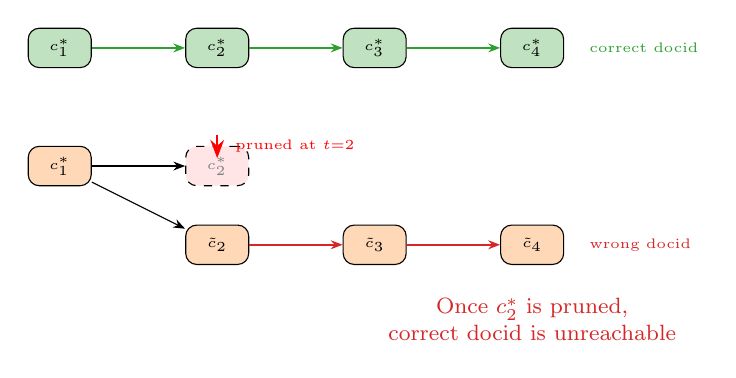
\begin{tikzpicture}[
    tok/.style={draw, rounded corners, fill=#1, minimum width=0.8cm, minimum height=0.5cm, font=\tiny},
    pruned/.style={draw, rounded corners, fill=red!10, dashed, minimum width=0.8cm, minimum height=0.5cm, font=\tiny, text=gray},
    arr/.style={-{Stealth[length=1.5mm]}, thin}
]
% Correct path
\node[tok=sealgreen!30] (c1) at (0, 1) {$c_1^*$};
\node[tok=sealgreen!30] (c2) at (2, 1) {$c_2^*$};
\node[tok=sealgreen!30] (c3) at (4, 1) {$c_3^*$};
\node[tok=sealgreen!30] (c4) at (6, 1) {$c_4^*$};
\draw[arr, sealgreen, thick] (c1) -- (c2);
\draw[arr, sealgreen, thick] (c2) -- (c3);
\draw[arr, sealgreen, thick] (c3) -- (c4);
\node[right=0.2cm of c4, font=\tiny, text=sealgreen] {correct docid};

% Beam path (error at step 2)
\node[tok=dsiorange!30] (b1) at (0, -0.5) {$c_1^*$};
\node[pruned] (b2) at (2, -0.5) {$c_2^*$};
\node[tok=dsiorange!30] (b2e) at (2, -1.5) {$\tilde{c}_2$};
\node[tok=dsiorange!30] (b3e) at (4, -1.5) {$\tilde{c}_3$};
\node[tok=dsiorange!30] (b4e) at (6, -1.5) {$\tilde{c}_4$};

\draw[arr] (b1) -- (b2);
\draw[arr] (b1) -- (b2e);
\draw[arr, hybridred, thick] (b2e) -- (b3e);
\draw[arr, hybridred, thick] (b3e) -- (b4e);
\node[right=0.2cm of b4e, font=\tiny, text=hybridred] {wrong docid};

% Annotation
\draw[thick, red, -{Stealth}] (2, -0.1) -- (2, -0.4) node[midway, right, font=\tiny, text=red, xshift=0.1cm] {pruned at $t{=}2$};

\node[below=0.3cm of b4e, font=\footnotesize, text=hybridred, align=center] {Once $c_2^*$ is pruned,\\correct docid is unreachable};
\end{tikzpicture}
\end{center}

\vspace{0.3cm}
\textbf{Probability of correct retrieval} (for beam width $B$ and ID length $L$):
\[
P(\text{correct}) \leq \left(1 - P(\text{prune at step } t)\right)^L
\]
Even small per-step error rates compound exponentially with ID length.
\end{frame}

\note{This is the fundamental beam search problem. If the correct token is pruned at any step, the correct docid becomes unreachable---there's no way to recover. With beam width $B$ and ID length $L$, even a small probability of pruning the correct token at each step compounds exponentially. This is why shorter document IDs are better (fewer chances for error) and why beam width matters so much.}

% ═══════════════════════════════════════════════
\section{The Role of Pre-training}
% ═══════════════════════════════════════════════

\begin{frame}[fragile]{Why Pre-training is Critical for Generative Retrieval}
\begin{center}
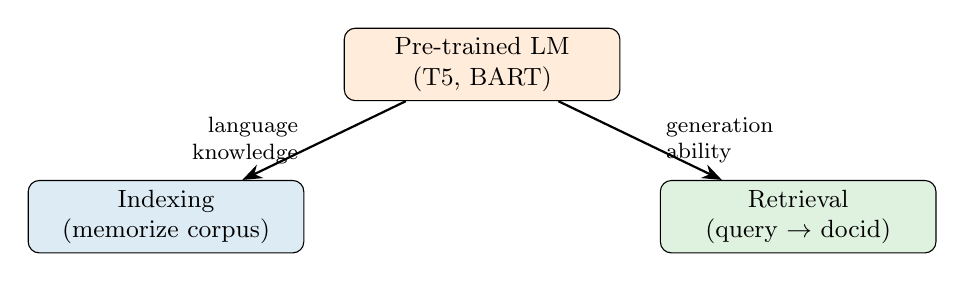
\begin{tikzpicture}[
    box/.style={draw, rounded corners, fill=#1, minimum height=0.7cm, minimum width=3.5cm, align=center, font=\small},
    arr/.style={-{Stealth[length=2.5mm]}, thick}
]
\node[box=dsiorange!15] (pretrain) {Pre-trained LM\\(T5, BART)};
\node[box=genreblue!15, below left=1cm and 0.5cm of pretrain] (index) {Indexing\\(memorize corpus)};
\node[box=sealgreen!15, below right=1cm and 0.5cm of pretrain] (retrieval) {Retrieval\\(query $\to$ docid)};

\draw[arr] (pretrain) -- (index) node[midway, left, font=\footnotesize, xshift=-0.2cm, align=right] {language\\knowledge};
\draw[arr] (pretrain) -- (retrieval) node[midway, right, font=\footnotesize, xshift=0.2cm, align=left] {generation\\ability};
\end{tikzpicture}
\end{center}

\vspace{0.3cm}
\textbf{Pre-training provides}:
\begin{enumerate}
    \item \textbf{Language understanding}: Semantic comprehension of queries and documents.
    \item \textbf{Memorization capacity}: Pre-training teaches models to store factual knowledge in parameters (``the world model'').
    \item \textbf{Generation fluency}: Coherent autoregressive generation of text-based IDs.
    \item \textbf{Zero-shot transfer}: Better generalization to unseen domains.
\end{enumerate}
\end{frame}

\note{Pre-training is essential for generative retrieval, even more so than for dense retrieval. It provides four things: language understanding (crucial for matching queries to documents), memorization capacity (the model has already learned to store facts), generation ability (needed for autoregressive ID production), and transfer learning (generalization to new domains). Without pre-training, generative retrieval essentially doesn't work at reasonable scale.}

% ═══════════════════════════════════════════════
\section{Evaluation \& Comparison with Dense Retrieval}
% ═══════════════════════════════════════════════

\begin{frame}{Performance Comparison: Generative vs.\ Dense}
\begin{center}
\begin{tabular}{lcccc}
\toprule
\textbf{Method} & \textbf{Type} & \textbf{NQ R@1} & \textbf{NQ R@10} & \textbf{MS MARCO MRR@10} \\
\midrule
BM25 & Sparse & 12.4 & 38.3 & 18.7 \\
DPR & Dense & 30.1 & 63.1 & 31.1 \\
ColBERT & Dense & 33.5 & 67.2 & 36.0 \\
\midrule
DSI (T5-base) & Generative & 27.4 & 56.6 & --- \\
GENRE & Generative & 35.2 & --- & --- \\
SEAL & Generative & 37.1 & 68.4 & --- \\
NCI & Generative & 51.5 & 77.9 & --- \\
LTRGR & Generative & 44.2 & 72.1 & 41.5 \\
\bottomrule
\end{tabular}
\end{center}

\vspace{0.3cm}
\textbf{Observation}: State-of-the-art generative methods are \emph{competitive with or surpass} dense retrieval on NQ. But the comparison is nuanced\ldots
\end{frame}

\note{Looking at the numbers, generative retrieval has caught up with and in some cases surpassed dense retrieval on Natural Questions. NCI's 51.5 R@1 is remarkable. However, these comparisons come with caveats: corpus size, evaluation protocol, and use of data augmentation vary across papers. The picture on MS MARCO (larger corpus) is less favorable for generative methods.}

\begin{frame}{When Does Generative Retrieval Win?}
\begin{center}
\begin{tabular}{p{4cm}cc}
\toprule
\textbf{Scenario} & \textbf{Generative} & \textbf{Dense} \\
\midrule
Static corpus, $< 1$M docs & \textcolor{sealgreen}{\checkmark} & \\
Dynamic corpus, frequent updates & & \textcolor{sealgreen}{\checkmark} \\
Web-scale ($> 100$M docs) & & \textcolor{sealgreen}{\checkmark} \\
End-to-end simplicity & \textcolor{sealgreen}{\checkmark} & \\
Sub-100ms latency required & & \textcolor{sealgreen}{\checkmark} \\
Zero-shot generalization & & \textcolor{sealgreen}{\checkmark} \\
Integration with LLMs (RAG) & \textit{emerging} & \textcolor{sealgreen}{\checkmark} \\
Interpretable retrieval & \textcolor{sealgreen}{\checkmark} & \\
\bottomrule
\end{tabular}
\end{center}

\vspace{0.3cm}
\textbf{Current consensus}: Dense retrieval for production systems at scale; generative retrieval for research and medium-scale applications.
\end{frame}

\note{The decision framework is clear. Generative retrieval wins when the corpus is static and manageable (under a million documents), when end-to-end simplicity matters, and when interpretability of the retrieval process is valued. Dense retrieval wins at scale, with dynamic corpora, and when latency is critical. For production search engines, dense retrieval with hybrid sparse+dense is the pragmatic choice today. Generative retrieval is an active research frontier with exciting potential.}

% ═══════════════════════════════════════════════
\section{Open Challenges \& Future Directions}
% ═══════════════════════════════════════════════

\begin{frame}{Open Research Questions}
\begin{enumerate}
    \item \textbf{Capacity theory}: Can we derive formal bounds on how many documents a model of size $|\theta|$ can memorize with retrieval accuracy $\geq 1 - \epsilon$?

    \vspace{0.15cm}
    \item \textbf{Optimal ID design}: Is there an information-theoretically optimal document ID scheme? What is the fundamental rate--distortion limit?

    \vspace{0.15cm}
    \item \textbf{Incremental learning}: How to add new documents without catastrophic forgetting? (cf.\ IncDSI)

    \vspace{0.15cm}
    \item \textbf{Scaling laws}: What is the precise relationship between model size, corpus size, and retrieval quality?

    \vspace{0.15cm}
    \item \textbf{Integration with LLMs}: Can large language models serve as generative retrievers in a RAG pipeline? How to separate retrieval from generation?

    \vspace{0.15cm}
    \item \textbf{Multimodal}: Extending beyond text --- GENIUS shows promise for image--text retrieval. Can we build unified multimodal generative retrievers?
\end{enumerate}
\end{frame}

\note{There are many exciting open questions. On the theory side: formal capacity bounds, optimal ID design, and scaling laws. On the practical side: incremental learning for dynamic corpora, integration with LLMs for RAG, and extension to multimodal retrieval. Each of these is an active research direction with papers appearing regularly.}

\begin{frame}[fragile]{The Bigger Picture: Retrieval in the Age of LLMs}
\begin{center}
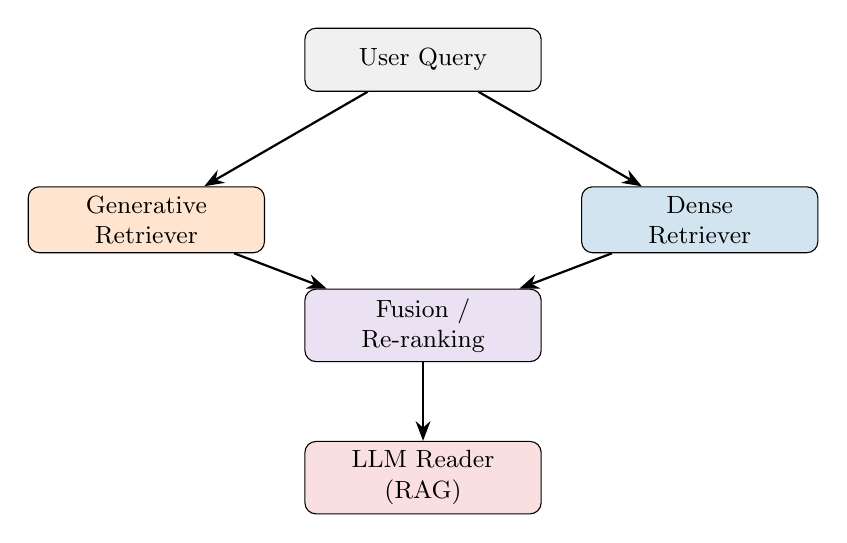
\begin{tikzpicture}[
    box/.style={draw, rounded corners, fill=#1, minimum height=0.8cm, minimum width=3cm, align=center, font=\small},
    arr/.style={-{Stealth[length=2.5mm]}, thick}
]
\node[box=lightgray] (q) {User Query};
\node[box=dsiorange!20, below left=1.2cm and 0.5cm of q] (gen) {Generative\\Retriever};
\node[box=genreblue!20, below right=1.2cm and 0.5cm of q] (dense) {Dense\\Retriever};
\node[box=ncipurple!20, below=2.5cm of q] (fuse) {Fusion /\\Re-ranking};
\node[box=hybridred!15, below=1cm of fuse] (llm) {LLM Reader\\(RAG)};

\draw[arr] (q) -- (gen);
\draw[arr] (q) -- (dense);
\draw[arr] (gen) -- (fuse);
\draw[arr] (dense) -- (fuse);
\draw[arr] (fuse) -- (llm);
\end{tikzpicture}
\end{center}

\vspace{0.2cm}
\textbf{Emerging paradigm}: Generative and dense retrieval as \emph{complementary} first-stage retrievers, feeding into LLM-based reading comprehension.
\end{frame}

\note{Looking ahead, the most promising direction may be combining generative and dense retrieval as complementary first-stage retrievers in a RAG pipeline. Generative retrieval captures global corpus structure; dense retrieval provides precise local matching. Together, they feed high-quality candidates to an LLM reader. This mirrors the general trend in AI: ensembles of diverse methods outperform any single approach.}

% ═══════════════════════════════════════════════
\section{Summary}
% ═══════════════════════════════════════════════

\begin{frame}{Key Takeaways}
\begin{enumerate}
    \item \textbf{Generative retrieval} encodes the corpus in model parameters and retrieves by \emph{generating} document identifiers.

    \vspace{0.15cm}
    \item \textbf{GENRE} pioneered constrained autoregressive generation with text-based entity IDs.

    \vspace{0.15cm}
    \item \textbf{DSI} established the two-phase (index + retrieve) framework with the docid design space.

    \vspace{0.15cm}
    \item \textbf{SEAL} uses natural-language n-grams as IDs, leveraging pre-trained LM knowledge via FM-Index.

    \vspace{0.15cm}
    \item \textbf{NCI} showed query augmentation is critical; \textbf{LTRGR} bridges generation and ranking.

    \vspace{0.15cm}
    \item \textbf{Theoretically}: Memorization capacity limits scalability; beam search errors compound; document ID design has an information-theoretic interpretation.

    \vspace{0.15cm}
    \item \textbf{Practically}: Competitive at medium scale ($<$1M docs); hybrid approaches needed beyond.
\end{enumerate}
\end{frame}

\note{To summarize: generative retrieval is a fundamentally new paradigm that treats retrieval as sequence generation. The key methods are GENRE, DSI, SEAL, and NCI. Document ID design is the central architectural question. Theory tells us that memorization capacity limits scalability, and beam search introduces compounding errors. In practice, generative retrieval is competitive at medium scale, and hybrid approaches bridge the gap to large-scale applications. This is a rapidly evolving field with many open questions.}

% ═══════════════════════════════════════════════
% REFERENCES
% ═══════════════════════════════════════════════

\begin{frame}[allowframebreaks]{References}
\footnotesize
\begin{itemize}
    \item Tay, Y.\ et al.\ (2022). Transformer Memory as a Differentiable Search Index. \textit{NeurIPS}.
    \item De Cao, N.\ et al.\ (2021). Autoregressive Entity Retrieval. \textit{ICLR}.
    \item Bevilacqua, M.\ et al.\ (2022). Autoregressive Search Engines: Generating Substrings as Document Identifiers. \textit{NeurIPS}.
    \item Wang, Y.\ et al.\ (2022). A Neural Corpus Indexer for Document Retrieval. \textit{NeurIPS}.
    \item Li, Y.\ et al.\ (2023). Multiview Identifiers Enhanced Generative Retrieval (MINDER). \textit{ACL}.
    \item Li, Y.\ et al.\ (2023). Learning to Rank in Generative Retrieval. \textit{AAAI}.
    \item Li, M.\ et al.\ (2024). Generative Dense Retrieval: Memory Can Be a Burden. \textit{arXiv:2401.10487}.
    \item Tang, Y.\ et al.\ (2024). From Matching to Generation: A Survey on Generative Information Retrieval. \textit{arXiv:2404.14851}.
    \item Kishore, R.\ et al.\ (2024). RIPOR: Optimization for Large-Scale Generative Retrieval. \textit{WWW}.
    \item Chen, J.\ et al.\ (2024). GENIUS: Generative Multi-Modal Retrieval. \textit{arXiv}.
    \item Arpit, D.\ et al.\ (2017). A Closer Look at Memorization in Deep Networks. \textit{ICML}.
    \item Lewis, M.\ et al.\ (2020). BART: Denoising Sequence-to-Sequence Pre-training. \textit{ACL}.
    \item Raffel, C.\ et al.\ (2020). Exploring the Limits of Transfer Learning with a Unified Text-to-Text Transformer (T5). \textit{JMLR}.
\end{itemize}
\end{frame}

\end{document}
